\newpage

\chapter{3D tisk}

Pro novou revizi desky byla navržena a vytištěna ochranná krabička, 
osazovací podložka a přípravek pro aplikaci pájecí pasty. 
Tyto prvky umožňují efektivní montáž, ochranu a zlepšení procesu výroby DPS. 

Konstrukce byla navržena pomocí online CAD softwaru \emph{Onshape}, 
což umožnilo rychlé iterace návrhu a snadné sdílení modelů.
 Výroba proběhla na \textit{3D} tiskárně \emph{Prusa Mk4}, 
 případně na jiném dostupném modelu tiskárny značky \emph{Prusa}. 

Všechny tištěné součásti využívají výplň \SI{15}{\percent} se vzorem \textit{3D Honeycomb}, 
která poskytuje optimální kombinaci pevnosti a úspory materiálu. 
Kromě toho byly aplikovány minimálně dva vnější vertikální perimetry 
a pět plných horizontálních vrstev na spodní straně, 
zatímco horní strana obsahuje čtyři plné vrstvy.
 Jako materiál byl zvolen \textit{PETG}, 
 který nabízí výbornou mechanickou odolnost, 
 tepelnou stabilitu a zároveň je vhodný pro ap	likace vyžadující pevnost a pružnost.

\section{Krabička}
Pro ochranu nové \textit{DPS}, bylo potřeba navrhnout krabičku s odnímatelným víkem.
Víko drží na krabičce pouze třením, to znamená bez použití zámků nebo šroubů.
Uvnitř krabičky se nachází 4 distanční sloupky, do kterých byly zataveny mosazné závity,
které umožňují spolehlivou, a opakovanou, montáž, či demontáž, DPS. 
Z boku a na víku krabičky jsou umístěny větrací otvory.
Jejich umístění a velikost byly zvoleny tak, aby se vzduch v krabičce pohyboval předvídatelným směrem.
Jinými slovy byla snaha o vytvoření airflow uvnitř krabičky a tím došlo ke vzniku optimálního chlazení.
Spodní řáda děr nacházejících se zboku krabičky by měla sloužit pro nasávání vzduchu pro chlazení spodní části desky MoSeZ.
Nasáty vzduch pak putuje kolem součástek na spodní straně DPS a ohřátý opouští krabičku otvory ve víčku.

\begin{figure}[H]
	\centering
	\includegraphics[width=0.75\linewidth]{kapitola3/figures/boxes_front.pdf}
	\caption{Krabičky pro MoSeZ}
	\label{priloha:boxes_front}
\end{figure}

\section{Osazovací podložka a přípravek pro aplikaci pájecí pasty}

Pro osazení byla využita automatická osazovačka \emph{OpenPnP}.
Osazovací automat vyžaduje, aby horní vrstva DPS byla ve výšce \SI{10}{\milli\meter} od pracovní desky. 
Návrh podložky tedy zohledňuje tloušťku samotné DPS a potřebnou výšku, aby osazování probíhalo správně. 
Podložka je pevně připevněna k pracovní desce osazovacího automatu 
a DPS se k ní uchycuje přes její montážní otvory.

\begin{figure}[H]
	\centering
	\includegraphics[width=0.75\linewidth]{kapitola3/figures/pap_holder.pdf}
	\caption{Držák DPS pro osazovačku}
	\label{priloha:pap_holder}
\end{figure}


Ke snadné aplikaci pájecí pasty byl navrhnut přípravek,
do kterého se upevní DPS a přes něj šablona.
Při aplikaci se šablona přitlačí na DPS 
a pomocí stěrky se nanese tenká vrstva pájecí pasty přes otvory v šabloně. 
Díky tomu je zajištěno, že pasta je aplikována pouze na pájecí plochy, 
čímž se minimalizuje riziko nežádoucích spojů a usnadňuje proces reflow pájení.

\begin{figure}[H]
	\centering
	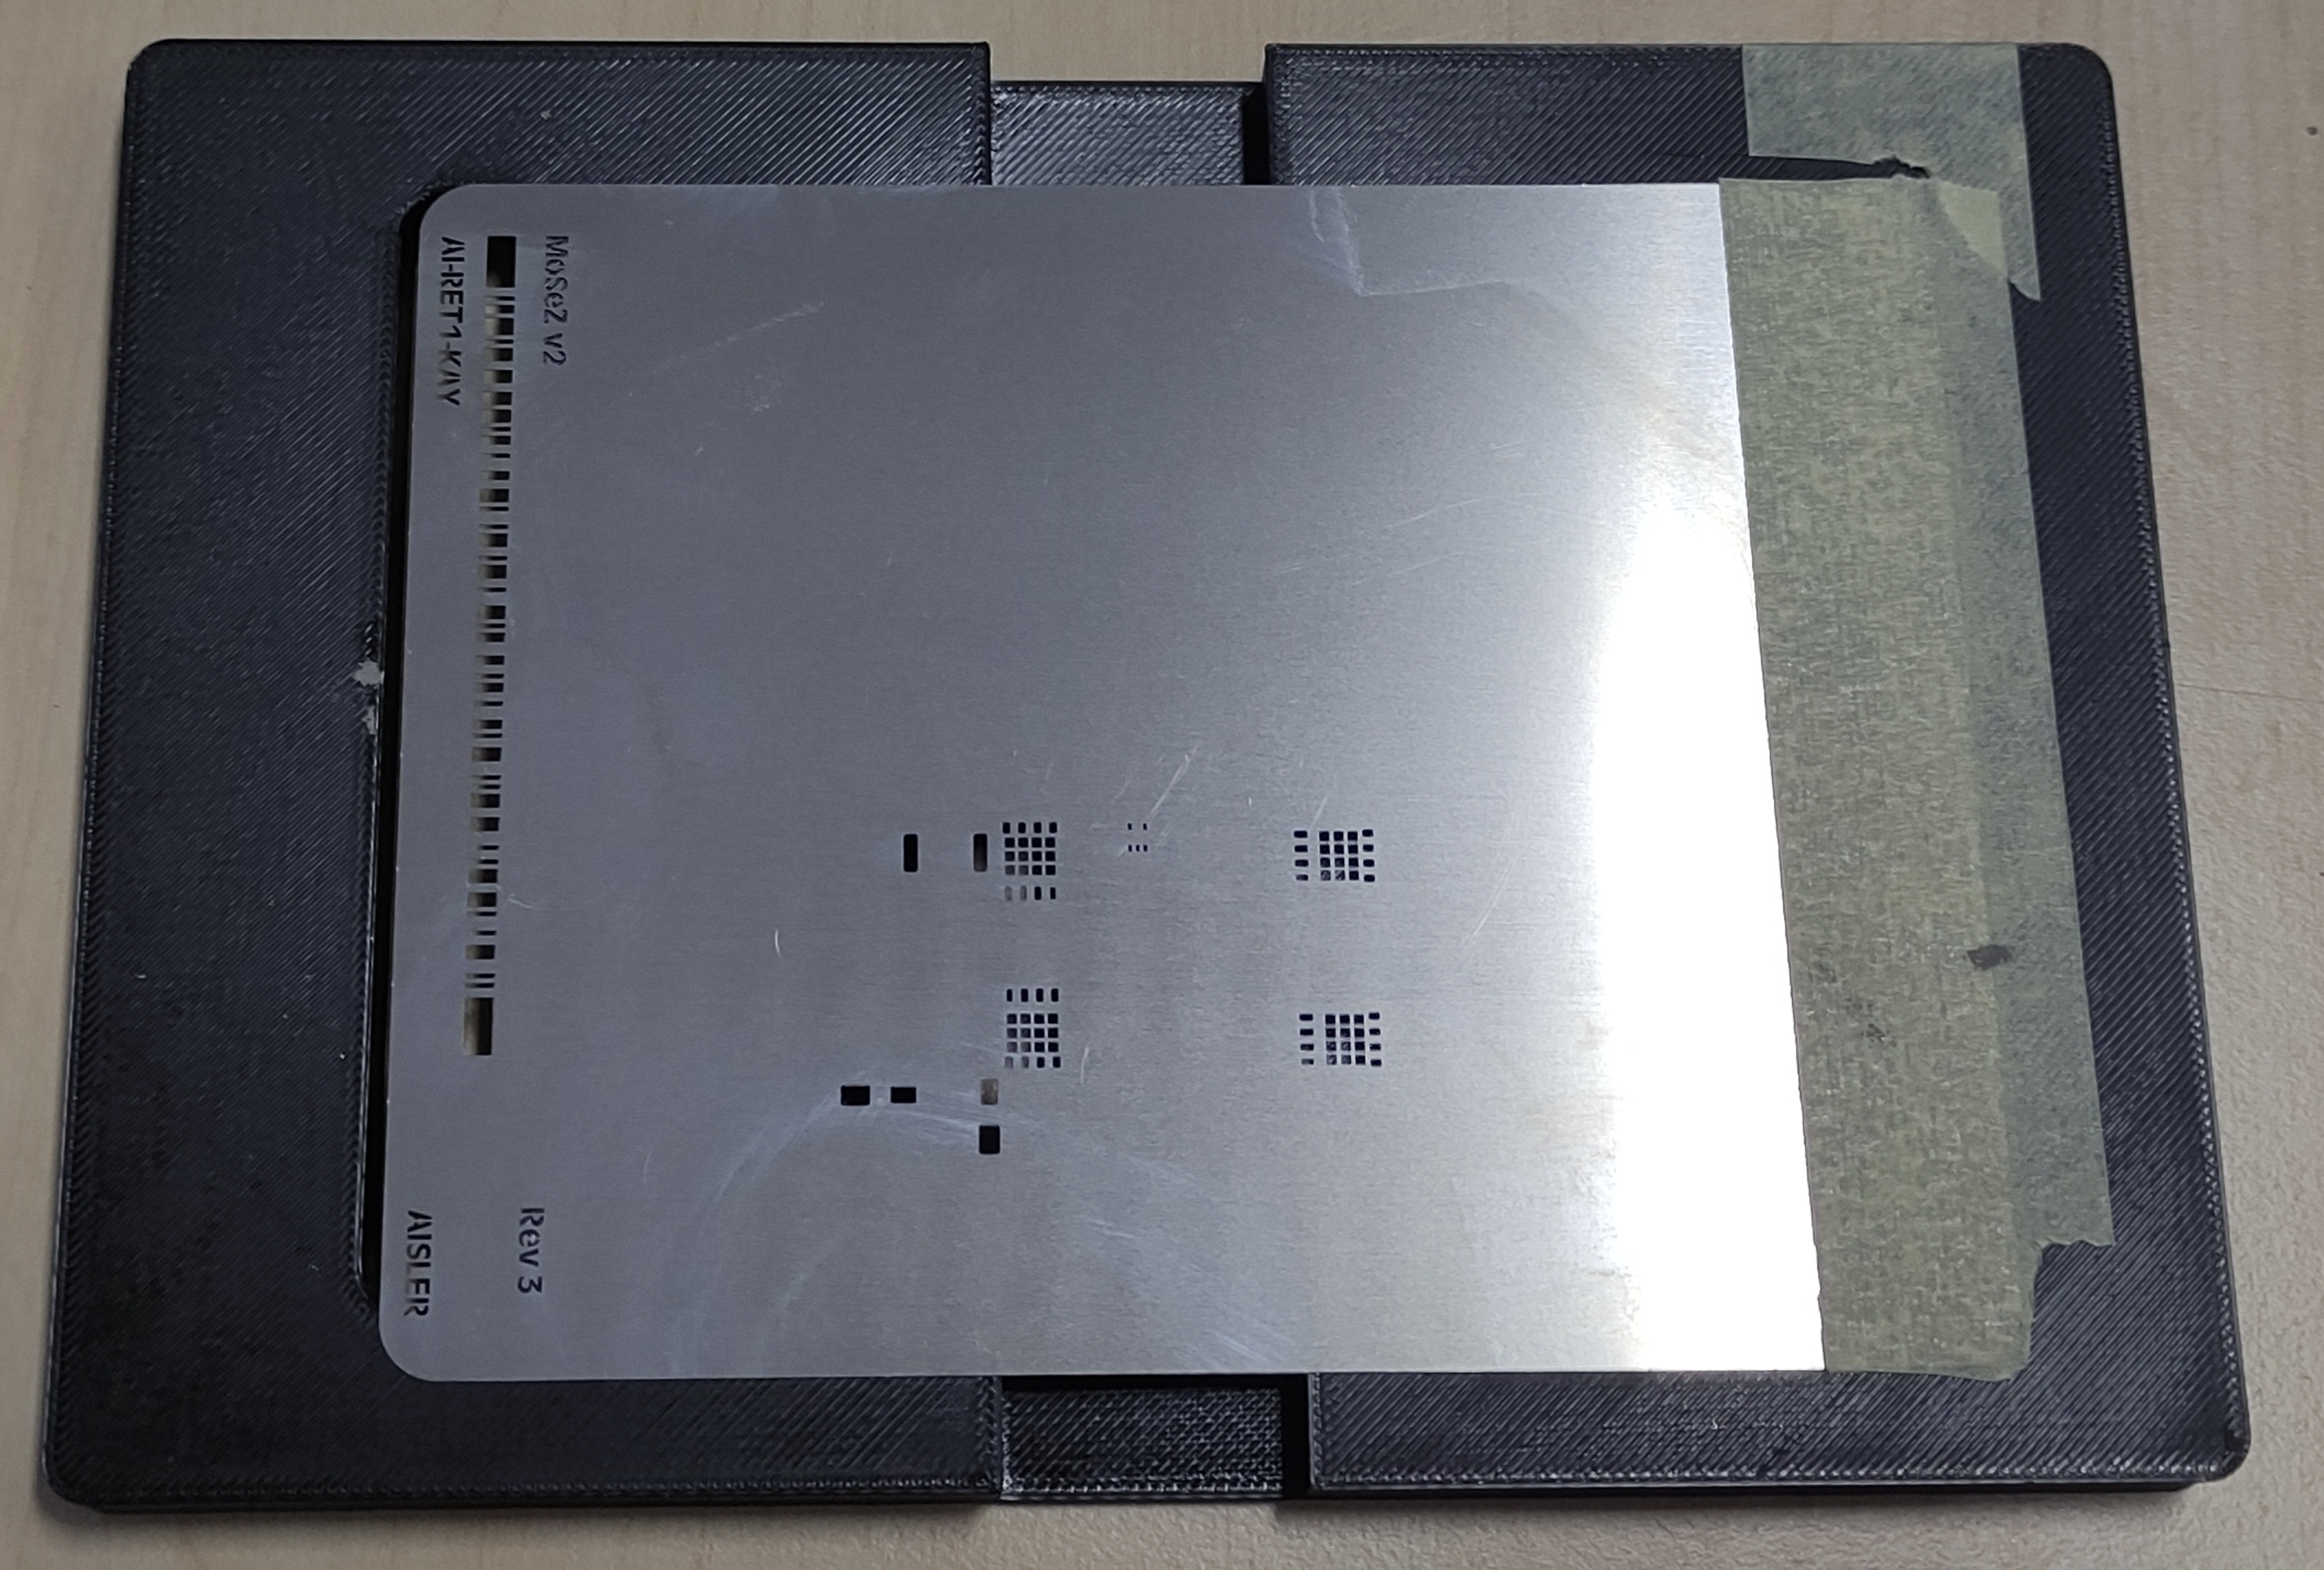
\includegraphics[width=\linewidth]{kapitola3/figures/paste_back.pdf}
	\caption{Držák DPS pro aplikaci pájecí pasty na zadní stranu DPS s již připevněnou šablonou}
	\label{priloha:paste_holder}
\end{figure}
